\setlength{\parskip}{\baselineskip}%
\setlength{\parindent}{0pt}%

In the winter of 1868/9, Swiss physician and biologist, Johannes Friedrich Miescher isolated an unknown substance from the nuclei of cells\cite{dahm2008discovering}. This substance was unlike anything he had observed before; it was resistant to protease, lacked sulphur, and contained large amounts of phosphorous. He recognised that he had isolated a novel substance and since it was isolated from the nucleus, he named it nuclein. Today, we know of this substance as nucleic acid (deoxyribonucleic and ribonucleic acid), the molecule of heredity.

Although Miescher speculated that nuclein may have had a role in heredity, he later rejected the idea. It wasn't until 1944, when Oswald Avery, Colin MacLeod, and Maclyn McCarty characterised the transforming factor in Griffith's Experiment\cite{griffith1928significance} as deoxyribonucleic acid (DNA), that it was hypothesised that DNA was the genetic material\cite{avery1944studies}. In order to identify DNA as the transforming factor, they used an enzyme that only degraded DNA (deoxyribonucleodepolymerase) and showed that it was able to eliminate the transforming power. It was later confirmed in 1952 by Alfred Hershey and Martha Chase that DNA was indeed the genetic material by performing a series of experiments in bacteriophages\cite{hershey1952independent}. They demonstrated that when bacteriophages infected bacteria, only their DNA would enter into the cytoplasm of the bacteria, whereas their protein would remain outside. This demonstrated that the genetic material that infected the bacteria was DNA.

Fast forward to the 21st century and not only have we sequenced the entire collection of DNA, the genome, of our very own species \cite{venter2001sequence, lander2001initial}, we have the capacity to sequence an entire human genome in a matter of days by using high-throughput sequencers. We have also just recently reached the \$1,000 genome era, whereby we can sequence the entire genome of an individual for around \$1,000 US dollars (USD). In contrast, the Human Genome Project, which gave us the first glimpse of the human genome costed approximately 2.7 billion fiscal year 1991 US dollars\cite{nhgri2010cost}. In just ~60 years, we have gone from establishing DNA as the molecule of heredity to being able to sequence a human genome in a few days for around 1,000 USD. Developments in molecular genetics is definitely moving at a very fast pace.

However, high-throughput sequencing is not limited to genome sequencing. The discovery of reverse transcriptase\cite{pmid4316300, pmid4316301} allowed the generation of complementary DNA (cDNA) from an ribonucleic acid (RNA) template; thus we are able to sequence the entire collection of RNA, known as the transcriptome, from biological samples. Other applications of sequencing allows us to capture genome-wide DNA-protein interactions, DNA methylation patterns, and histone modifications\cite{applicationsofsequencing}. Many of these applications are named with a ``Seq" suffix; for example RNA-Seq refers to RNA sequencing and ChIP-Seq refers to chromatin immunoprecipitation sequencing. There is a large number of *Seq protocols\cite{pachter2014seq}, and this number will definitely increase with the decrease in the cost of sequencing.

This thesis focuses primarily on the study of transcriptomes; while the genome is assumed to be more or less identical in the ~37 trillion cells that make up the human body\cite{pmid23829164}, transcriptomes in different cells and tissues are different. It is the differential use of the genome that is thought to give rise to over 400 different cell types that make up a human\cite{pmid16790079}. However differential usage may also be an indication of disease; transcriptomes isolated from cancerous cells are quite different from normal cells. By comparing transcriptomes we can gain insight into the molecular processes that define different cell types or drive a cell to becoming cancerous. In this work, we have studied the transcriptomes of different biological systems. The first paper examined a particular type of bias that arose in the use high-throughput transcriptome profiling and demonstrated how such biases can be mitigated\cite{Tang01022013}. The second paper was a study investigating the role of small RNAs in the DNA damage response (DDR), employing small RNA sequencing to identify a new class of small RNA implicated in DDR\cite{francia2012site}. The third paper was a study on human induced pluripotent stem cells (iPSCs) and the use of transcriptome profiling to explore the role of a certain chemokine in iPSCs. The fourth paper focused on a particular class of DNA known as repetitive elements (REs) and investigated the RNA expression patterns of such elements. The fifth paper was a study involving the profiling of RNA in whole blood and how transcriptome profiling could be a useful tool for finding biomarkers. The sixth and last paper investigates a particular class of small RNA known as piwi-interacting RNA (piRNA) and proposes a role of piRNAs in Rett syndrome.

\section{History of DNA and genes}

The classical definition of a gene dates back to Gregor Mendel when he demonstrated in his plant breeding experiments that discrete traits could be inherited from parents to offspring. While the mechanism of inheritance wasn't clear at that time, these heritable traits were termed a gene. The definition of a gene has evolved with our increasing knowledge of genetics and biochemistry\cite{pmid17567988}. The idea that genes were blueprints for proteins was perceived when mutations in Neurospora genes could cause defects in steps in metabolic pathways\cite{pmid16578042}. This became the ``one gene, one polypeptide" hypothesis; the idea was that each gene was responsible for producing a single enzyme/protein in a biochemical pathway. The association of DNA with genes began with Griffith's Experiment\cite{griffith1928significance}, where it was demonstrated that heritable traits could be transferred between dead and live bacteria. It was later demonstrated that this heritable material was DNA\cite{avery1944studies}.

DNA was discovered by Johannes Friedrich Miescher who subsequently named it nuclein. In 1881, Albrecht Kossel determined that nuclein was composed of five bases: adenine (A), cytosine (C), guanine (G), thymine (T), and uracil (U) and in 1889, Richard Altmann discovered that nuclein was acidic and renamed it as nucleic acid. The basic component of DNA was deduced by Phoebus Levene in 1909, where he discovered that DNA consisted of an acid, an organic base, and a sugar; he also showed that these components were linked together as phosphate-sugar-base to form units, which he termed nucleotides. This sugar-phosphate backbone forms the structural framework of nucleic acids. While Levene proposed that DNA was made up equal amounts of A, C, G, and T, it was discovered by Erwin Chargaff that DNA should have a 1:1 ratio of pyrimidine (C, T, and U) and purine (A and G) bases, which is known as Chargaff's rules. Chargaff's rules was one of the observations that led to the eventual deduction of the three-dimensional (3D) structure of DNA.

The 3D structure of DNA showed how adenines paired with thymines and cytosines paired with guanine\cite{WATSON_1953}; this is now known as Watson-Crick base pairing (Figure ~\ref{fig:dna}). The base pairing explained how genetic information could be copied as they famously wrote in their paper:

\epigraph{``It has not escaped our attention that the specific pairing we have postulated immediately suggests a possible copying mechanism for the genetic material."}{--- \textup{Watson and Crick}}

\begin{figure}[h]
   \centering
   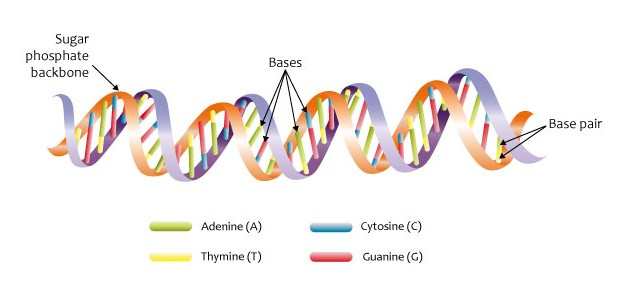
\includegraphics[width=\textwidth,natwidth=625,natheight=307]{dna.jpg}
   \caption[The structure of DNA]{The structure of DNA is based on the repeated pattern of a sugar and phosphate group, known as the sugar phosphate backbone, and the base pairing of the four bases, adenine (A), cytosine (C), guanine (G), and thymine (T). Image by NHS National Genetics and Genomics Education Centre licensed under the Creative Commons license.}
   \label{fig:dna}
\end{figure}

The relationship between DNA and proteins was demonstrated by the use of artificial ribonucleic acid (RNA) and bacterial cells\cite{pmid14471390}. RNA is synthesised by RNA polymerase, using DNA as a template, which is a process known as transcription. By using RNA artificially created to be composed of entirely uracils, Matthaei and colleagues produced a protein composed entirely of the amino acid phenylalanine. This experiment demonstrated that nucleic acids contained a code for amino acids. This code, known as the genetic code, was later cracked three years later\cite{pmid5330357} and defined how information is encoded in the genetic material. Nirenberg and colleauges worked out that three nucleotides defined a codon and is translated into one of the 20 standard amino acids. This flow of information from nucleic acid to protein was described as the ``Central Dogma"\cite{crick1958protein}.

At that period of time, a gene was known as a section of DNA that was used in the production a particular protein. In each gene, the nucleotides were arranged in a specific order to facilitate the production of the corresponding amino acids and eventual protein. However with the advent of DNA sequencing and high-throughput sequencing, the definition of a gene further evolved.

\section{DNA sequencing}

Determining the exact order of nucleotides in DNA

Early efforts at sequencing genes were very labour intensive.

\subsection{Sanger and Maxam-Gilbert sequencing}

Two of the earliest protocols for DNA sequencing were chain-termination/dideoxy sequencing\cite{pmid271968}, which was also known as Sanger sequencing, and chemical sequencing\cite{pmid265521}, which was also known as Maxam-Gilbert sequencing. These two methods, which were developed in the 1970s, are considered to be the first generation of DNA sequencing methods. Both methods require the use polyacrylamide gel electrophoresis, which can resolve DNA fragments at a 1 bp resolution, for determining the DNA bases. However, the generation of the DNA fragments is different between the two methods.

The key feature of Sanger sequencing is the use of dideoxynucleotide triphosphates (ddNTPs) and a purified DNA polymerase enzyme to synthesise DNA. The structure of a normal nucleotide (dNTP), consists of a 3' hydroxyl (OH) group in the pentose sugar. The chain-terminating ddNTPs lack the OH group that is necessary for the formation of the phosphodiester bond between one nucleotide and the next during DNA strand elongation. If a ddNTP is incorporated into a growing DNA strand, the strand elongation is terminated. The idea is to set up a reaction with a mixture of dNTPs [deoxyadenosine triphosphate (dATP), deoxyguanosine triphosphate (dGTP), deoxycytidine triphosphate (dCTP), deoxythymidine triphosphate (dTTP)] and one particular ddNTP in a ratio of 300:1. Most of the times, the DNA will be elongated but once the ddNTP is incorporated the strand stops. This results in a number of DNA fragments of varying lengths and depending on the ddNTP used, the last base of the fragment corresponds to that base. This reaction is carried out for the other ddNTPs and all the fragments are separated using polyacrylamide gel electrophoresis. By reading the ladder, the DNA bases can be deduced.

The Maxam-Gilbert sequencing method relies on the use of chemicals that can cleave specific bases. Dimethyl sulfate is used to cleave purine bases (A and G) and hydrazine is used to cleave pyrimidine bases (C and T). To distinguish the purines, an adenine-enhanced cleavage step is carried out, which cleaves adenines preferentially. To distinguish the pyrimidines, NaCl is used with hydrazine to suppress the reaction of thymines. As with Sanger sequencing, the DNA fragments are separated using polyacrylamide gel electrophoresis, and the DNA bases are deduced by reading the gel.

\subsection{Second generation sequencing}

Automation of Sanger sequencing by using radioactively or fluorescently labeled ddNTPs.

Shendure et al., \cite{pmid15143316}

\section{The human genome}

Inside every somatic nucleated cell in the human body are 23 pairs of chromosomes; these chromosomes make up the human genome. A chromosome is a long DNA molecule that is condensed so that it may physically fit inside the nucleus (Figure ~\ref{fig:dna_condensed}). We can estimate the physical length the human genome by multiplying the number of base pairs contained on each chromosome by the length of a base pair. The haploid human genome contains ~3\e{9} base pairs of DNA; therefore there is a total of 6 billion base pairs of DNA per cell. Given that each base pair of DNA is ~0.34 nanometers long or 3.4\e{-10} meters\cite{pmid7354864}, each diploid cell contains 3.4\e{-10} * 3\e{9} * 2 or 2.04 meters of DNA. Given that the estimated number of cells in the human body is around 3.7\e{13} or 37 trillion\cite{pmid23829164}, a typical person contain ~74 trillion meters of DNA. Certain proteins, called histones, help compact the vast amounts of DNA inside of us (specifically, inside the eukaryotic nucleus). The histones are a family of small, positively charged proteins that provide the energy, in the form of electrostatic interactions, to fold negatively charged DNA (due to the phosphate groups in its phosphate-sugar backbone). The resulting DNA-protein complex is called chromatin.

\begin{figure}[h]
   \centering
   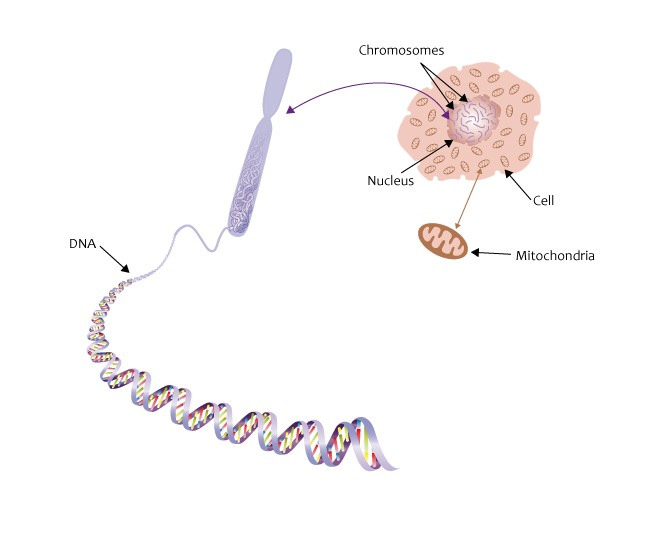
\includegraphics[width=\textwidth,natwidth=650,natheight=539]{dna_condensed.jpg}
   \caption[Condensation of DNA]{DNA is condensed into chromosomes by forming DNA-protein complexes known chromatin, which is further coiled into thicker fibers called 30nm fibers. The chromosomes reside inside the nucleus of a cell. Mitochondria also contain its own DNA. Image by NHS National Genetics and Genomics Education Centre licensed under the Creative Commons license.}
   \label{fig:dna_condensed}
\end{figure}

Chromatin possesses a fundamental repeating structure\cite{holde01111974}, known as nucleosomes and the packaging of DNA into nucleosomes shortens DNA about sevenfold. However despite this, chromatin is still too long to fit inside the nucleus, which is ~10 to 20 microns in diameter. Chromatin is further coiled into a thicker fiber, called the 30nm fiber, because it is roughly 30 nanometers in diameter. Processes such as transcription and replication require the two strands of DNA to come apart temporarily, thus allowing polymerases access to the DNA template. However, the presence of nucleosomes and the folding of chromatin into 30-nanometer fibers pose barriers to the enzymes that unwind and copy DNA. It is therefore important for cells to have means of opening up chromatin fibers and/or removing histones transiently to permit transcription and replication to proceed. Generally speaking, there are two major mechanisms by which chromatin is made more accessible:

\begin{enumerate}
   \item Histones can be enzymatically modified by the addition of acetyl, methyl, or phosphate groups.
   \item Histones can be displaced by chromatin remodelling complexes, thereby exposing underlying DNA sequences to polymerases and other enzymes.
\end{enumerate}

It is important to remember that these processes are reversible, so modified or remodelled chromatin can be returned to its compact state after transcription and/or replication are complete.

\section{Applications of sequencing}

The age of high throughput sequencing and the application of this technology to studying the transcriptome (also epigenome and interactome)

\subsection{Transcriptomics}

The transcriptome is the collection of RNA molecules derived from the genome at a particular time and location. The diversity of cells is determined by the expression patterns of genes and transcription factors (TFs).

\subsection{Transcription}

The genome is a store of biological information but requires the coordinated activity of enzymes and proteins to bring about transcription. Chromatin structure and nucleosome positioning are altered in order for the transcriptional machinery to access parts of the genome for transcription. The pre-initiation complex that contains RNA polymerase II and general transcription factors forms near the core promoter region around the transcription start site and primes RNA polymerase II for transcription. Processing of precursor RNA include the addition of a cap and poly-A tail, splicing, and RNA editing. Removal of the cap is considered to the first step towards mRNA degradation. The capping procedure is thought to occur only in the nucleus, however a cytoplasmic form of a capping enzyme has been identified; the role of cytoplasmic re-capping.

\begin{itemize}

   \item The transcription preinitiation complex (PIC) positions the polymerase over the transcription start site
   \item The PIC binds at the promoter, which contains binding sites for the PIC
   \item Classification of promoters depend on the distance from the TSS, core, proximal, and distal promoter
   \item The TATA box is a sequence that contains a TA-rich pattern about 30 bp upstream from the TSS
   \item The TATA binding protein (TBP) binds to the TATA box and is involved in DNA strand separation during transcription
   \item Core promoter elements include the initiator element (Inr), the downstream promoter element (DPE), the TFIIB recognition element (BRE) and the CpG island (CGI)

\end{itemize}

\begin{figure}[h]
   \centering
   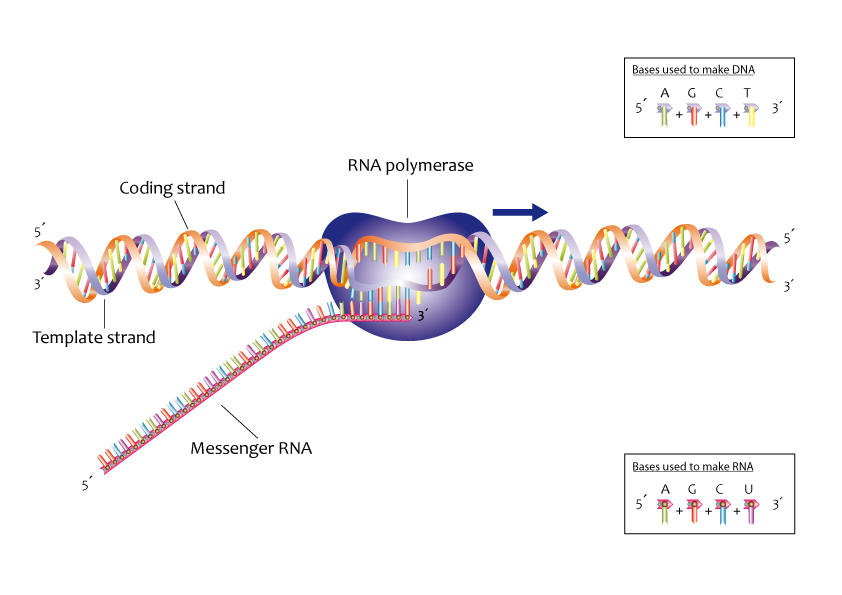
\includegraphics[width=\textwidth,natwidth=842,natheight=595]{transcription.jpg}
   \caption[DNA transcription]{The process of transcription begins with RNA polymerase, which reads the DNA sequence (the template strand) in the 5' to 3' direction and produces a complementary RNA strand called the messenger RNA (mRNA). The mRNA has the same sequence as the coding strand, except that thymines are replaced by uracils. Image by NHS National Genetics and Genomics Education Centre licensed under the Creative Commons license.}
   \label{fig:transcription}
\end{figure}

\subsection{RNA polymerase}

The genetic information encoded in DNA is transcribed into RNA by RNA polymerases.

\subsection{Reverse transcription}

\begin{itemize}

   \item Studies on the yeast transcriptome using DNA microarrays showed that although mRNAs are being degraded and re-synthesised all the time, the composition of the yeast transcriptome undergoes very little change if the environment remains constant
   \item However on switching from aerobic to anaerobic respiration, the levels of over 700 mRNAs increase by a factor of two or higher, and another 1,000 mRNAs decline to less than half their original amount
   \item Studying the transcriptome of acute lymphoblastic leukemia cells with respect to acute myeloid leukemia cells revealed differences that made it possible to distinguish the two types of leukemia
   \item Collection of full length cDNAs by the FANTOM consortium revealed many transcripts of unknown function (TUFs)
   \item The technologies that allowed full length cDNA sequencing
   \item Cap Analysis Gene Expression (CAGE) for genome-wide identification of transcription start sites
   \item Biotinylation of diol groups of RNA (High Efficiency Selection of Full-length cDNA by Improved Biotinylated Cap Trapper)
   \item PacBio sequencing has read lengths greater than 10kb and can be used for full length cDNA sequencing

\end{itemize}

\section{The repetitive genome}

Since the release of the draft human genome sequence\cite{venter2001sequence, lander2001initial}, it was established that only a small fraction of the genome is made up of protein-coding sequences and the majority of the genome was made up with repetitive elements. As the human genome contains the entire instruction set that is necessary for the development of a human, the decoding of the genome was thought to provide answers to many outstanding biological questions. However, there are several paradoxes that are still currently unresolved:

\begin{enumerate}
   \item K-value paradox: complexity does not correlate with the number of chromosomes
   \item C-value paradox: complexity does not correlate with genome size
   \item N-value paradox: complexity does not correlate with the number of protein coding genes
\end{enumerate}

If we measure organismal complexity in terms of mental cognition, we observe that complexity is not correlated to the number of chromosomes, the size of genomes, and the number of protein coding genes. Humans have 46 chromosomes and some species of butterflies have over hundreds of chromosomes, such as \textit{Polyommatus atlantica}. In terms of genome size, the species \textit{Polychaos dubium}, a freshwater amoeboid, has one of the largest genomes known with ~670 gb of DNA sequence; humans on the other hand have a genome size of ~3 gb. And lastly humans have roughly the same number of protein-coding genes as \textit{Caenorhabditis elegans}, ~20,000 versus ~21,000, respectively. However, the \textit{C. elegans} genome is ~100 mb\cite{celegans1998sequencing}, which is ~30 times smaller than the human genome, despite having a similar number of genes. One of the discrepancies between genome sizes despite having a similar number of genes is due to repetitive elements, which makes up roughly 50\% of the human genome. Among 66 vertebrate genomes, the percentage coverage of repetitive elements in the human genome is quite high (Figure ~\ref{fig:repeat_coverage_vertebrate_genome}).

\begin{figure}[h]
   \centering
   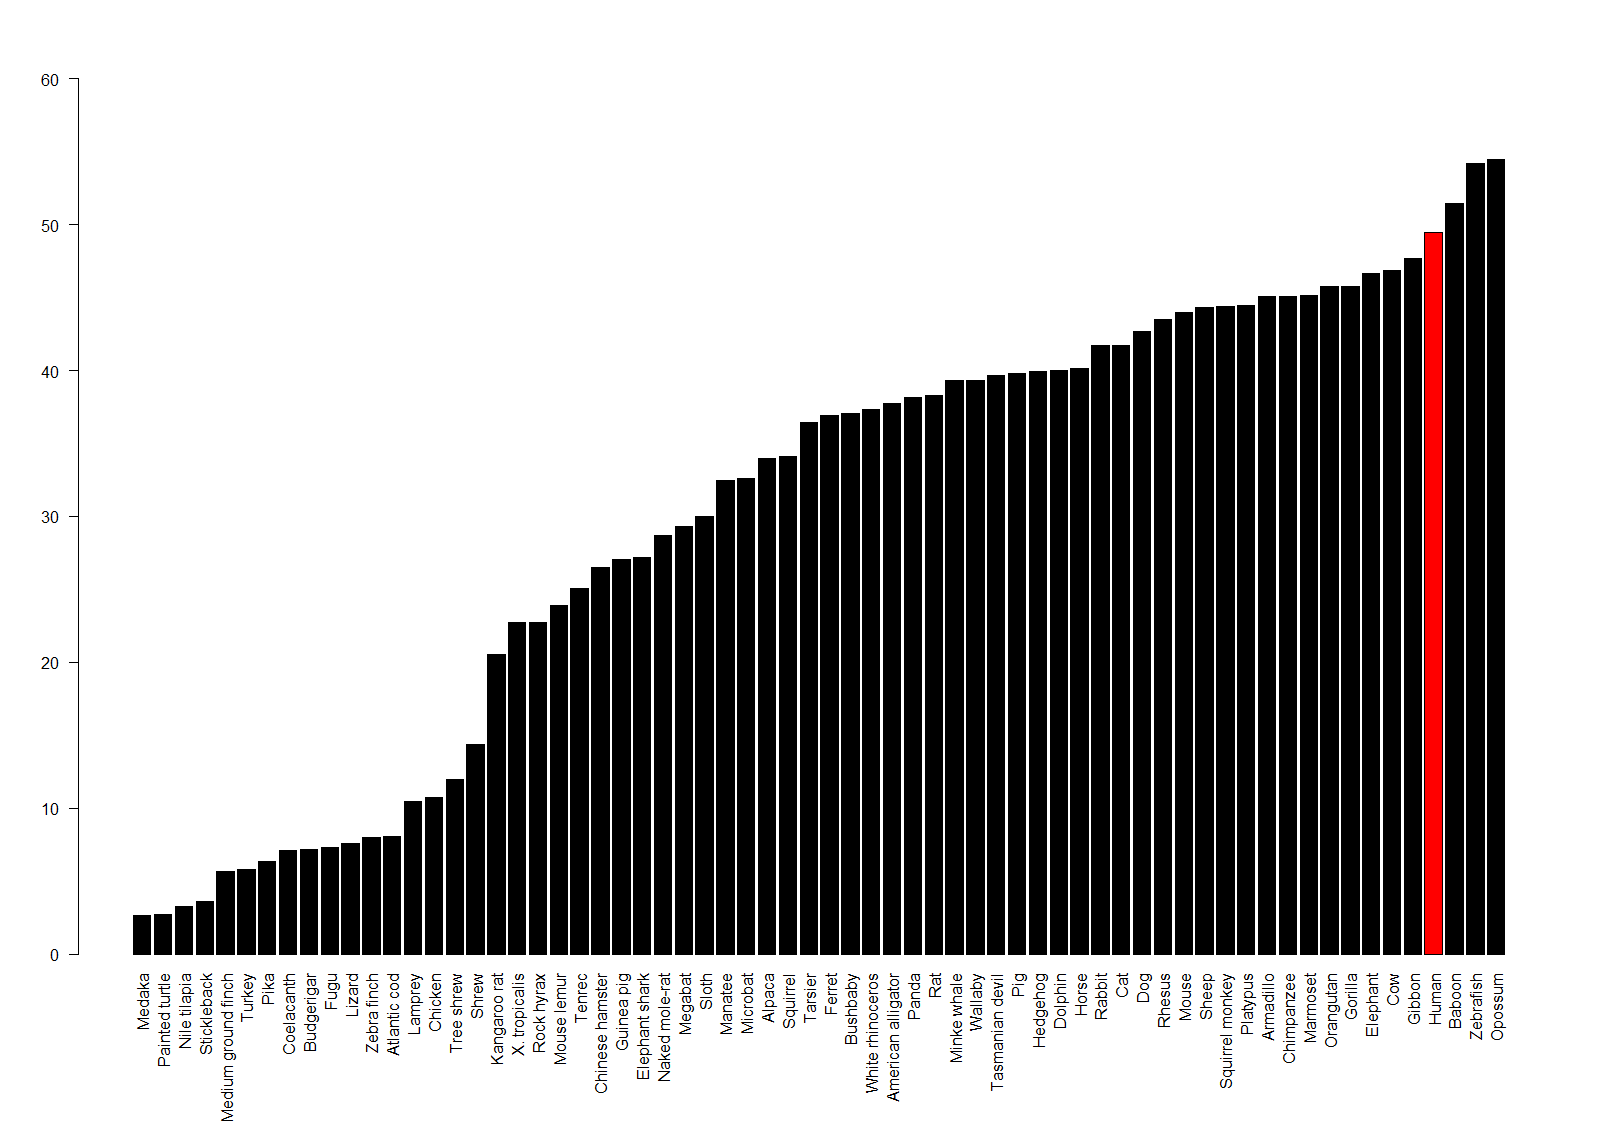
\includegraphics[width=\textwidth,natwidth=1600,natheight=1148]{repeat_coverage_vertebrate_genome.png}
   \caption[Coverage of repetitive elements in vertebrate genomes]{The total coverage of repetitive element in 66 vertebrate genomes as annotated by RepeatMasker in the respective genomes\cite{tang2014repcoverage}.}
   \label{fig:repeat_coverage_vertebrate_genome}
\end{figure}

However, the larger vertebrate genomes do not always contain the highest percentage of repetitive elements (Figure ~\ref{fig:genome_size}). At least in humans, transposons make up the majority of the repetitive elements that make up the human genome. In particular class I transposons (retrotransposons), which are able to transcribed and inserted into the genome, make up a large portion of the human genome. W.Ford Doolittle and Carmen Sapienza wrote in 1980\cite{doolittle1980selfish}: ``When a given DNA, or class of DNAs, of unproven phenotypic function can be shown to have evolved a strategy (such as transposition) which ensures its genomic survival, then no other explanation for its existence is necessary" and Leslie Orgel and Francis Crick, wrote that junk DNA has little specificity and conveys little or no selective advantage to the organism\cite{orgel1980selfish}.

The origin of the term ``junk DNA" is usually attributed to Susumu Ohno, who used it to describe pseudogenes, which are gene copies that have no known biological function. In its modern day usage, ``junk DNA" is used to describe DNA sequence that goes not play a functional role in an organism. Dr. Ohno estimated that there would be an upper limit to the number of functional loci in mammalian genomes based on mutational load and a fixed mutation rate. He predicted that mammalian genomes could not have more than 30,000 loci under selection as this would guarantee a progressive decline in fitness, leading to extinction.

\begin{figure}[h]
   \centering
   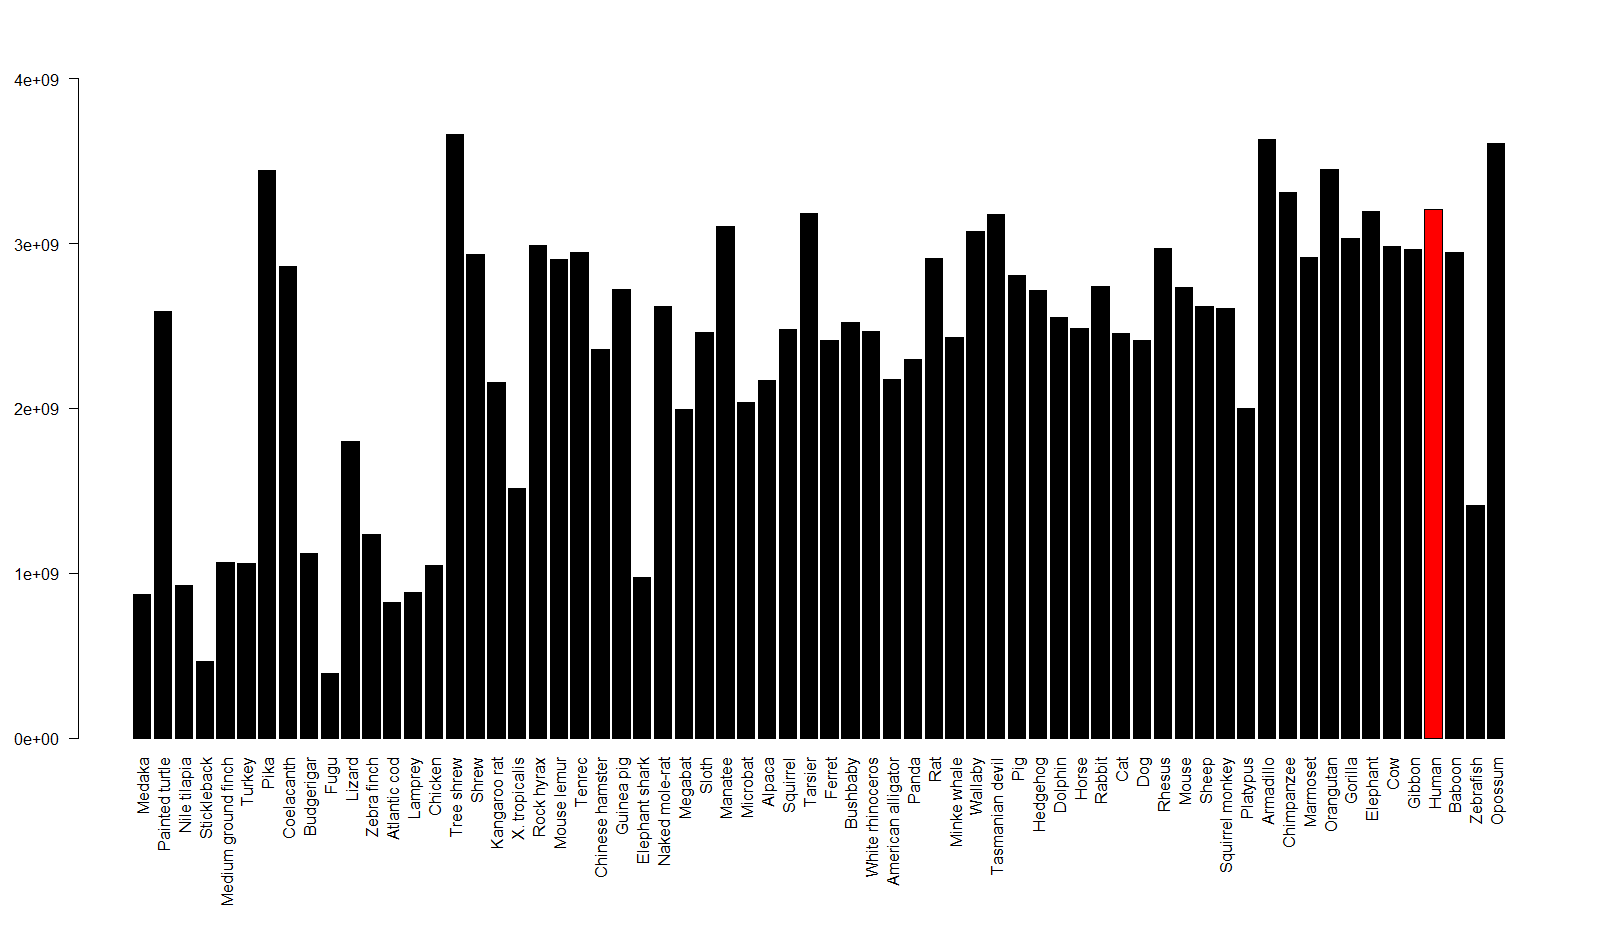
\includegraphics[width=\textwidth,natwidth=1600,natheight=932]{genome_size.png}
   \caption[Vertebrate genomes sizes]{The genome sizes of 66 vertebrate genomes, sorted from the lowest to highest percent of repetitive element coverage\cite{tang2014gensize}.}
   \label{fig:genome_size}
\end{figure}

\begin{figure}[h]
   \centering
   \includegraphics[width=9cm, angle=270]{barplot_repeat_family.eps}
   \caption[Tally of repetitive element families in the hg19 genome]{The number of repetitive element families determined by RepeatMasker in the hg19 genome.}
   \label{fig:repeat_family}
\end{figure}

\begin{itemize}
   \item Messenger RNAs are transcripts of protein-coding genes and are translated into protein
   \item Classical non-coding RNA found in both prokaryotes and eukaryotes are ribosomal RNAs and transfer RNAs, which are both involved in protein synthesis
   \item Diverse class of non-coding RNAs, broadly broken down into long and short non-coding RNA
   \item Assembly of non-coding RNAs with proteins as ribonucleoprotein (RNP) structures
   \item Interaction of non-coding RNAs with chromatin
   \item Pervasive transcription describes the observation that a large percentage of DNA in mammalian genomes is transcribed.
   \item Tiling arrays and full length cDNA sequencing suggested that most of the genome is transcribed
   \item The ENCODE pilot project provided multiple lines of evidence that most of the mammalian genome is associated with at least one primary transcript, i.e., pervasive transcription of the genome
   \item Are the majority of detected low-level transcription due to technical artifacts and/or background biological noise?
   \item Protocols that capture only poly-A transcripts as opposed to poly-A minus and cytoplasmic versus nuclear enrichment libraries
   \item Sequencing depth and sampling of RNA molecules; absolute transcript quantification will help (such as using unique molecule identifiers and non-PCR based methods)
   \item Functional transcriptomics in the post-ENCODE era, specifically what is the criteria for functionality
   \item Repeat-associated binding sites (RABS) are over-represented in proximity of regulated genes and that the binding motifs within these repeats have undergone evolutionary selection
   \item Indeed, studies conducted both at the gene and genome levels have uncovered TE insertions that seem to have been co-opted - or exapted - by providing transcription factor binding sites (TFBSs) that serve as promoters and enhancers, leading to the hypothesis that TE exaptation is a major factor in the evolution of gene regulation.
   \item The transcription of repetitive elements, especially transposable elements, in specific tissues
   \item Repetitive elements are usually highly methylated, however differentiation methylation patterns of repetitive elements was observed in specific tissues
   \item Functions of some GWAS candidates in intergenic regions (such as http://www.nature.com/nature/journal/v507/n7492/full/nature13138.html)
\end{itemize}

\section{Stem cells}

\begin{itemize}
   \item Stem cells have two key characteristics that make them different from other cells
   \item They can reproduce themselves for long periods of time; this is known as self-renewal and
   \item They can differentiate or specialise into specific cell types under certain conditions
   \item Embryonic stem cells are derived from the inner cell mass of blastocysts. In normal development, the inner cell mass begins growing into all the different cell types of the fully developed body
   \item In our fully developed bodies, we have some self-renewing cells that reside in a specific tissue that are able to generate specific types of differentiated cells, i.e., they have limited differentiation ability. They were named adult stem cells because they reside in fully formed tissues.
   \item However, some adult stem cells have a transdifferentiation ability, which is that they can generate cells outside their own tissue type.
   \item They are also known as somatic stem cells or tissue stem cells.
   \item Haematopoietic stem cells (HSCs), which are somatic stem cells, reside in the medulla of the bone (bone marrow) and have the unique ability to give rise to all of the different mature blood cell types and tissues.
\end{itemize}
